\documentclass[runningheads]{llncs}

\usepackage[T1]{fontenc}
\usepackage{graphicx}
% \renewcommand\UrlFont{\color{blue}\rmfamily}
\usepackage{hyperref}
\usepackage{color}
\usepackage{setspace}
\usepackage{verbatim}
\usepackage{multicol}
\usepackage{array}
\newcommand{\PreserveBackslash}[1]{\let\temp=\\#1\let\\=\temp}
\newcolumntype{C}[1]{>{\PreserveBackslash\centering}p{#1}}
\newcolumntype{R}[1]{>{\PreserveBackslash\raggedleft}p{#1}}
\newcolumntype{L}[1]{>{\PreserveBackslash\raggedright}p{#1}}
\setlength{\tabcolsep}{3pt}

\renewcommand{\floatpagefraction}{0.9}
\renewcommand{\textfloatsep}{2.0ex}
\renewcommand{\dbltextfloatsep}{2.0ex}

\newenvironment{packed_itemize}{
\vspace*{-0.5em}
\begin{itemize}
\setlength{\partopsep}{0pt}
\setlength{\itemsep}{1pt}
\setlength{\parskip}{0pt}
\setlength{\parsep}{0pt}
}{\end{itemize}}

\begin{document}

\title{An Empirical Assessment of Progress in ATP}
\titlerunning{Progress in ATP}

\author{
Geoff Sutcliffe\inst{1}\orcidID{0000-0001-9120-3927}
\and
Christian Suttner\inst{2}
\and \\
C. Raymond Perrault\inst{3}\orcidID{0009-0001-1178-343X}
\and \\
Lars Kotthoff\inst{4}\orcidID{0000-0003-4635-6873}
\and \\
Zain~Khalid\inst{1}\orcidID{0009-0001-2063-6933}
}
\authorrunning{G. Sutcliffe, et al.}
\institute{University of Miami, USA,
\email{geoff@cs.miami.edu},
\email{zsk17@miami.edu}
\and
Deceased
\and 
SRI International, USA,
\email{ray.perrault@sri.com}
\and 
University of Wyoming, USA,
\email{larsko@uwyo.edu}
}

\maketitle
%--------------------------------------------------------------------------------------------------
\begin{abstract}
The TPTP World is a well established infrastructure that supports research, development, and 
deployment of Automated Theorem Proving (ATP) systems
Data in the TPTP World has been used to assess progress in ATP in the last decade, in
terms of 
first solutions of problems that are of direct interest to humans, 
the fraction of unsolved problems, 
the fraction of easy problems,
decreasing problem difficulty ratings, 
and 
temporal Shapley values.
The analyses show WHAT?

\keywords{Automated Theorem Proving \and Empirical Evaluation \and Progress in ATP}
\end{abstract}
%--------------------------------------------------------------------------------------------------
\section{Introduction}
\label{Introduction}

The TPTP World \cite{Sut17} is a well established infrastructure that supports research, 
development, and deployment of Automated Theorem Proving (ATP) systems.
The TPTP World includes the TPTP problem library,
% \cite{Sut09}, 
the TSTP solution library,
% \cite{Sut10}, 
standards for writing ATP problems and reporting ATP solutions,
% \cite{SS+06,Sut08-KEAPPA}, 
tools and services for processing ATP problems and solutions,
% \cite{Sut10}, 
and it supports the CADE ATP System Competition (CASC).
% \cite{Sut16}.
Various parts of the TPTP World have been deployed in a range of applications,
in both academia and industry.
The web page \href{https://www.tptp.org}{\tt www.tptp.org} provides access to all 
components.

Any meaningful assessment of progress in ATP must refer to the ability of systems to solve 
ATP problems.
As the ATP systems are improved over time, the problems that they must solve also change to meet 
the demands of applications.
(If there is a fixed set of problems then the systems can simply be finely tuned to solve that
fixed set, with inevitable asymptotic progress towards solving all the problems.)
The TPTP problem library provides an evolving set of ATP problems that reflect the needs of 
ATP users, and is an appropriate basis for assessing the changing ability of ATP systems.
Alongside the TPTP problem library, the TSTP solution library provides data about ATP 
systems' abilities to solve the problems in the TPTP problem library.
This paper examines the progress in ATP, based on the data from TPTP v6.3.0 released on 
28th November 2015 to TPTP v8.2.0 released on 13th June 2023.
Five analyses are considered:
(i)~First ATP solutions of individual problems that are of direct interest to humans;
(ii)~The fraction of unsolved problems over fixed coherent sets of problems;
(iii)~The fraction of easy problems over fixed coherent sets of problems;
(iv)~The decrease in problem difficulty ratings over fixed coherent sets of problems;
(v)~Shapley values over time and at fixed points in time.
All five analyses are fundamentally based on the ability of ATP systems to solve TPTP problems, and 
do not explicitly factor in the resources needed to find solutions, e.g., hardware, time limits, 
etc. 
Section~\ref{ResourceLimits} explains why this makes sense in the ATP context.

The use of system performance data to evaluate a field of endeavour is common.
In the realm of logic-based systems, examples include
the various compititions \cite{BB+19} for logic-based systems, e.g., CASC \cite{Sut16}, the SAT 
Competition \cite{JL+12}, SMT-COMP \cite{BdS05,CSW15}, the ASP Competition \cite{CI+12},
the Technical Performance chapter of Stanford University's AI Index Annual Report \cite{MF+23},
the use of Shapley values to evaluate algorithmic improvements in SAT solving \cite{FK+16,KF+19},
and
an examination of progress in SAT solving comparing algorithmic and hardware advances \cite{FHS20}.
A general examination of the requirements for such benchmarking is provided by \cite{BLW19}.
In all cases the common features of the evaluation are (i)~the ability of systems solve given test
problems, and (ii)~the resources required by the systems to solve those test problem.
In order for the results to be relevant, the test problems must be representative of the problems
the systems will face in applications, and the resource measurements must be appropriate for 
the availability and demands of the applications.

It is important to differentiate between evaluations at instances in time, such as provided by
competitions, and evaluation over time.
At instances of time the test problems used for evaluation, the systems being evaluated, and
the hardware/software platform used, are static.
That provides a clean basis for detailed comparison between systems.
In contrast, evaluation over time is complicated by changing test problems, changing systems,
and changing hardware/software.
This dynamic evaluation environment requires additional control to provide meaningful results.

\paragraph{Paper structure:}
Section~\ref{TPTP} provides ...
Section~\ref{TSTP} provides ...
Section~\ref{AnalysisProcesses} provides ...
Section~\ref{Evidence} provides ...
Section~\ref{Conclusion} concludes. 

%--------------------------------------------------------------------------------------------------
\section{The TPTP Problem Library}
\label{TPTP}

The core of the TPTP World is the TPTP problem library \cite{Sut09}; it is the de facto standard 
set of test problems for classical logic ATP systems.
The problems can be browsed online\footnote{%
\href{https://www.tptp.org/cgi-bin/SeeTPTP?Category=Problems}
{\tt www.tptp.org/cgi-bin/SeeTPTP?Category=Problems}}
and documentation is available\footnote{%
\href{https://www.tptp.org/cgi-bin/SeeTPTP?Category=Documents}
{\tt www.tptp.org/cgi-bin/SeeTPTP?Category=Documents\&File=OverallSynopsis}}.
Each release of the problem library is identified by a number in the form 
$version$.$edition$.$patch$.
The $version$ is incremented when important new features are added,
the $edition$ is incremented when new problems are added, and
the $patch$ is incremented when errors have been corrected.
The current release is v8.2.0.
Section~\ref{TSTP} explains why the analyses of progress presented in this paper start at
TPTP~v6.3.0.
Table~\ref{TPTPReleases} gives some summary data about the TPTP releases from v6.3.0 to v8.2.0.
The Size column gives the number of problems in the release to the time of the release, while
the Analysed column gives the number of problems left for analysis after the data cleaning 
described in Section~\ref{AnalysisData}.
The acronyms for problem types are listed in Section~\ref{SPCs}.

\begin{table}[htb]
\begin{center}
\setlength{\tabcolsep}{4pt}
\begin{tabular}{ll|l|rr}
Release & Date     & Changes                                 & Size & Analysed \\
\hline
% v6.2.0  & 14/07/15 & TSTP data from StarExec                 &   20654 & 20012 \\
v6.3.0  & 28/11/15 & New TFO problems with arithmetic        &   20762 & 20168 \\
v6.4.0  & 31/06/16 & New problems                            &   20897 & 20839 \\
v7.0.0  & 24/07/17 & First TH1 problems                      &   21851 & 21310 \\
v7.1.0  & 06/03/18 & TXF syntax specified                    &   22011 & 21893 \\
v7.2.0  & 10/07/18 & New problems                            &   22026 & 21909 \\
v7.3.0  & 02/08/19 & New problems                            &   22686 & 22570 \\
v7.4.0  & 10/07/20 & New problems                            &   23291 & 23118 \\
v7.5.0  & 13/07/21 & New problems                            &   24098 & 24027 \\
v8.0.0  & 19/04/22 & First TXF problems                      &   24785 & 24027 \\
v8.1.0  & 30/07/22 & New problems                            &   25257 & 25103 \\
v8.2.0  & 13/06/23 & New problems                            &   25474 & 25325 \\
\end{tabular}
\end{center}
\caption{Overview of TPTP releases}
\label{TPTPReleases}
\end{table}

Each TPTP problem file has a header section (as comments) that file contains information for users
in four parts:
the first part identifies and describes the problem;
the second part provides information about occurrences of the problem in the literature and 
elsewhere;
the third part provides semantic and syntactic characteristics of the problem;
the last part contains comments and bugfix information.
The third part is most relevant to this work. 
It contains the problem's SZS status \cite{SZS03} that provides the semantic status of the 
problem, e.g., if it is a {\tt Theorem}, a {\tt Satisfiable} set of formulae, a problem whose 
status is {\tt Unknown}, etc.
It also contains statistics about the problem's syntax, e.g., the number of formulae, the 
number of predicate and functions symbols, the use of connectives, etc.
The SZS status and the syntactic characteristics are used to form the Specialist Problem Class
of the problem.

%--------------------------------------------------------------------------------------------------
\subsection{Specialist Problem Classes}
\label{SPCs}

The problems in the TPTP library are divided into Specialist Problem Classes (SPCs) -- classes of 
homogeneous problems with the same recognizable logical, language, and syntactic characteristics.
% SPCs added in v4.1.0 15/06/10
Evaluation of ATP systems within SPCs makes it possible to say which systems work well for what 
types of problems. 
The appropriate level of subdivision for SPCs is that at which less subdivision would merge 
SPCs for which ATP systems have distinguishable behaviour, and at which further subdivision
would unnecessarily split an SPC for which ATP systems have reasonably homogeneous behaviour.
Empirically, this is ensured by examining the patterns of system performance across the 
problems in each SPC. 
For example, the separation of ``essentially propositional'' problems was motivated by observing 
that SPASS (WA+99) performed differently on the ALC problems in the SYN domain of the TPTP.
A data-driven test of the homogeneity can also provide assurance that the SPCs are
appropriate \cite{FS02}.

The characteristics used to define the SPCs in TPTP v8.2.0 are~\ldots
\begin{enumerate}
\item TPTP language: \\
      {\tt CNF} -- Clause Normal Form
      {\tt FOF} -- First-Order Form \\
      {\tt TF0} -- Typed Monomorphic First-order form \\
      {\tt TF1} -- Typed Polymorphic First-order form \\
      {\tt TX0} -- Typed Monomorphic eXtended First-order form \\
      {\tt TX1} -- Typed Polymorphic eXtended First-order form \\
      {\tt TH0} -- Typed Monomorphic Higher-order form \\
      {\tt TH1} -- Typed Polymorphic Higher-order form
\item SZS status: \\
      {\tt THM} (includes {\tt CAX}) -- Theorem (includes Contradictory AXioms) \\
      {\tt CSA} -- CounterSAtisfiable \\
      {\tt UNS} -- UNSatisfiable \\
      {\tt SAT} -- SATisfiable \\
      {\tt OPN} -- OPeN  \\
      {\tt UNK} -- UNKown
\item Order (for {\tt CNF} and {\tt FOF}): \\
      {\tt PRP} -- PRoPositional \\
      {\tt EPR} -- Effectively PRopositional (known to be reducible to {\tt PRP}) \\
      {\tt RFO} -- Real First-Order (not known to be reducible to {\tt PRP})
\item Equality: \\
      {\tt NEQ} -- No EQuality \
      {\tt EQU} -- EQUality (some or pure) \\
      {\tt SEQ} -- Some (not pure) EQUality \\
      {\tt PEQ} -- Pure EQUality (for {\tt CNF}: either {\tt UEQ} or {\tt NUE}) \\
      {\tt UEQ} -- Unit EQUality \\
      {\tt NUE} -- Non-Unit Equality
\item Hornness (for {\tt CNF}): \\
      {\tt HRN} -- HoRN
      {\tt NHN} -- Non-HorN
\item Arithmetic (for {\tt T*} languages): \\
      {\tt NAR} -- No ARithmetic \\
      {\tt ARI} -- ARIthmetic.
\end{enumerate}

Using these characteristics 223 SPCs are defined in TPTP v8.2.0.
Some examples are:
{\tt CNF\_SAT\_EPR\_PEQ\_UEQ} -- clause normal form satisfiable clauses that are effectively
propositional, have purely equality literals in unit equality clauses;
{\tt FOF\_THM\_RFO\_SEQ} -- first-order theorems that are ``really first-order'' (not known
to be effectively propositional), and contain some (not only) equality;
{\tt TF0\_THM\_NEQ\_ARI} -- typed monomorphic first-order theorems that have no equality but do
include arithmetic.
Combinations of SPCs are written using UNIX globbing, e.g., {\tt TF0\_THM\_*\_NAR} is the
combination of {\tt TF0\_THM\_EQU\_NAR} and {\tt TF0\_THM\_NEQ\_NAR} -- typed monomorphic 
higher-order theorems problems, either with or without equality, but no arithmetic.

The SPCs are used when computing the TPTP problem ratings.

%--------------------------------------------------------------------------------------------------
\subsection{TPTP Problem Ratings}
\label{Ratings}

Each TPTP problem has a difficulty rating that provides a well-defined measure of how difficult 
the problem is for current ATP systems \cite{SS01}.
The ratings are based on performance data in the TSTP (see Section~\ref{TSTP}), and are updated
in each TPTP edition.
Rating is done separately for each SPC.
A partial order between systems is determined according to whether or not a system solves a strict 
superset of the problems solved by another system. 
If a strict superset is solved, the first system is said to {\em subsume} the second system. 
The union of the problems solved by the non-subsumed systems defines the state-of-the-art -- all 
the problems that are solved by any system. 
The fraction of non-subsumed systems that fail on a problem is the difficulty rating for the 
problem. 
Problems that are solved by all of the non-subsumed systems get a rating of 0.00 (``easy'');
problems that are solved by some of the non-subsumed systems get a rating between 
0.00 and 1.00 (``difficult''); 
problems that are solved by none of the non-subsumed systems get a rating of 1.00 (``unsolved'').

%--------------------------------------------------------------------------------------------------
\section{The TSTP Solution Library}
\label{TSTP}

The complement of the problem library is the TSTP solution library \cite{Sut07-CSR,Sut10}.
% Started as the results collection for the TPTP circa 1997, became the TSTP circa 2002.
The TSTP is built by running all the ATP systems that are available in the TPTP World on
all the problems in the TPTP problem library.
The ATP systems come from a range of sources:
some were developed many years ago, and are no longer distributed;
some are the most recent available, taken either from the systems’ web sites or from the most 
recent edition of CASC.
At the time of writing this paper, the TSTP contained the results of running 87 ATP systems and 
system variants on all the problems in the TPTP that they could attempt.
% (therefore, e.g., systems that do model finding for FOF are not run on THF problems).
This has produced 1091026 runs, of which 432718 (39.6\%) solved the problem.
One use of the TSTP is for ATP system developers to examine solutions to problems and thus 
understand how they can be solved, leading to improvements to their own systems. 
The use considered here is as the basis for TPTP problem ratings.

% User hardware at first, moved to my servers around 2010, then StarExec Iowa \cite{SST14} in 2012,
Prior to 2010 the data in the TSTP came from results submitted by ATP system developers, who
performed testing on their own hardware.
From 2010 to 2013 the data was generated on the TPTP World servers at the University of Miami.
Since 2014 the ATP systems have been run on StarExec \cite{SST14}, initially on the StarExec
Iowa cluster, and since 2018 on the StarExec Miami cluster.
StarExec has provided stable platforms that produce reliably consistent and comparable data in
the TSTP.
The analyses presented in Section~\ref{AnalysisProcesses} start at TPTP v6.3.0, which was released 
in November 2015. 
By that time the problem ratings were consistently and reliably based on data produced on the 
StarExec computers.

The StarExec Iowa computers have an 
quad-core Intel(R) Xeon(R) CPU E5-2609 CPU run at 2.40 GHz,
128 GiB memory,
and the CentOS Linux release 7.9.2009 (Core) operating system
Linux kernel 3.10.0-693.el7.x86\_64.
The StarExec Miami computers have an
octa-core Intel(R) Xeon(R) E5-2667 v4 CPU run at 2.10 GHz,
128 GiB memory,
and the CentOS Linux release 7.4.1708 (Core) operating system
Linux kernel 3.10.0-1160.62.1.el7.x86\_64.
One ATP system is run on one CPU at a time, with a 300s CPU time limit and a 128GiB memory
limit (see Section~\ref{ResourceLimits}).
The minor differences between the Iowa and Miami configurations can be ignored for the task
of ``solving problems'', as is explained in Section~\ref{ResourceLimits}.

%--------------------------------------------------------------------------------------------------
\subsection{Resource Limits}
\label{ResourceLimits}

Analysis shows that increasing resource limits does not significantly affect which problems 
are solved by each ATP system. 
Figure\ref{PPPPlot} illustrates this point; it plots the CPU times taken by several contemporary 
ATP systems to solve the TPTP problems for the SPCs {\tt FOF\_THM\_RFO\_*}, in increasing order 
of time taken. 
The data was taken from the TSTP, i.e., using the StarExec Miami computers.
The relevant feature of these plots is that each system has a point at which the time taken to 
find solutions starts to increase dramatically. 
This point is called the system's Peter Principle \cite{PH69} Point (PPP), as it is the point at 
which the system has reached its level of incompetence. 
Evidently a linear increase in the computational resources beyond the PPP would not lead to the 
solution of significantly more problems. 
The PPP thus defines a realistic computational resource limit for the system. 
From an ATP perspective, the PPP is the point at which the ATP system gets lost in its quickly 
growing search space. 
Even though there may be enough memory to represent the search space at the PPP, the system is 
largely unable to find a solution within the space. 
The point thus also defines a realistic memory resource limit. 
Therefore, provided that enough CPU time and memory are allowed for an ATP system to reach its 
PPP, a usefully accurate measure of what problems it can solve within realistic resource limits 
is achieved.
The performance data in the TSTP is produced with adequate resource limits.

\begin{figure}[ht!]
\centering
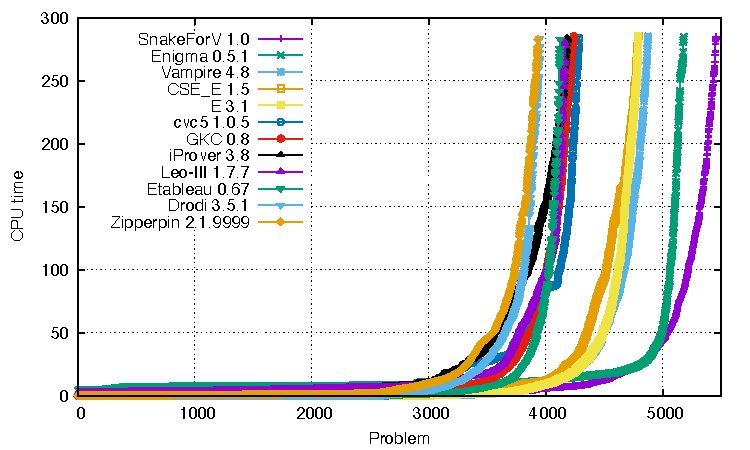
\includegraphics[width=0.75\textwidth]{Plots/FOF_THM_RFO_PPP/FOF_THM_RFO_PPP}
\vspace*{-1em}
\caption{CPU times for {\tt FOF\_THM\_RFO\_*}}
\label{PPPPlot}
\end{figure}

%--------------------------------------------------------------------------------------------------
\section{Analysis Processes}
\label{AnalysisProcesses}

%--------------------------------------------------------------------------------------------------
\subsection{Analysis Data}
\label{AnalysisData}

The analyses performed in this assessment use the TPTP problem ratings, and historical data about 
which ATP systems solved which problems in each TPTP release.
The data was extracted from the {\tt ProblemAndSolutionStatistics} file that accompanies each TPTP 
release, which summarizes information from the header fields of the TPTP problem files and
corresponding TSTP solution files.
As explained in Section~\ref{TSTP}, TSTP data starting from TPTP v6.3.0 in November 2015 has been
used, taking snapshots at each TPTP edition up to v8.2.0.

Before analysis the rating data was cleaned as follows:

\paragraph{Cleaning for Bias:}
The TPTP tags problems that are designed specifically to be suited or ill-suited to some ATP 
system, calculus, or control strategy as {\em biased}. 
This includes the {\tt SYN000} problems, which are designed for test ATP systems' parsers.
The biased problems are excluded from the analyses.

\paragraph{Cleaning for Bugfixes:}
Over time there are problems that have to be removed from the TPTP because they are renamed,
duplicates, wrongly formulated, etc.
Such problems in a TPTP release are thus not in subsequent releases.
The removed problems are excluded from the analyses.

\paragraph{Cleaning for the Past:}
Problems are added to the TPTP in each release, and corresponding TSTP data is generated using 
the available ATP systems.
As it is not possible to run all previously available ATP systems on new problems when they 
are added to the TPTP, it was (quite reasonably) assumed that if a problem is unsolved by the 
current ATP systems when it is added to the TPTP, then it would have been unsolved by 
previously available ATP systems.
The rating data was thus augmented for problems added after v6.3.0 with an initial rating 
of 1.00 (unsolved), by setting the problems' ratings in prior TPTP releases to 1.00.
This, however, can lead to an unfairly optimistic view of progress, because those retrospectively 
added 1.00 ratings increase the average problem rating in the past.
For problems added after v6.3.0 with an initial rating less than 1.00, it is unknown if the
previously available ATP systems would have been able to solve them.
Augmenting the rating data by setting the problems' ratings in prior TPTP releases to their 
initial rating can lead to a pessimistic view of progress, because those retrospectively
added ratings decrease the average problem rating in the past.
The optimistic/pessimistic effect gets stronger when rating data is augmented for problems that
were added in more recent TPTP releases.
In this work the rating data was augmented for all problems added after v6.3.0.
That results in 4486 problems having their ratings augmented, 1854 by 1.00 and 2632 by less than 
1.00.

\paragraph{Cleaning for Change:}
A counterintuitive feature of an individual problem's difficulty ratings is that they sometimes 
increase with time, because they are computed wrt the TSTP data from all the currently available
ATP systems.
Increases are caused by new ATP systems (or system versions) becoming available.
If a new system is not subsumed then its TSTP data is used in the rating process.
The ratings of problems that the new system solves decrease, but at the same time the ratings of
problems that the new system does not solve increase\footnote{%
Conversely, if a system that was not subsumed becomes unavailable, it does not contribute TSTP
data for new problems.
The new problems have higher ratings than they would have had if the system had remained
available.
Since the TSTP data started being generated on StarExec, this has been a rare occurrence, e.g.,
Isabelle ran fine on StarExec Iowa, but did not port to StarExec Miami in 2018.
This has not materially impacted the analyses of progress.} -- you have to ``pay the piper''.
A common case of this phenomenon is a new system that can solve some previously unsolved
(rating 1.00) problems, but that cannot solve a substantial number of problems that are solved
by other systems (rating less than 1.00).
An increase of a problem's rating is counterintuitive because the problem has not changed, and 
it could still be solved by the previously available systems.
This anomaly was noted in prior analysis \cite{Sut17} where it was noted: ``The ratings generally 
show a downward trend - there has been progress!'', but ``ratings can also increase when data 
from new systems is added to the TSTP.''
In this work the anomaly is resolved by additionally looking at {\em monotonic ratings}:
if a problem's rating in a TPTP release is greater than it's previous rating, the monotonic 
rating is set to the previous lower rating.
Monotonized ratings make clear sense in the case of problem that was unsolved (rating 1.00) and 
is then solved by a new system (the rating drops to less than 1.00) -- if a problem is 
solved, it cannot become unsolved -- the solving system still exists in principle.
In cases where the rating is less than 1.00 monotonized ratings might considered to be 
optimistic, because ratings do have to ``pay the piper''.

%--------------------------------------------------------------------------------------------------
\subsection{Coherent SPC Sets}
\label{SPCSets}

Four of the analyses performed (see Section~\ref{AnalysisTypes}) use the data for a set of 
problems.
In order for such analyses to be meaningful it is necessary for the problems in each set to be 
reasonably coherent, so that the analysis results are wrt that type of problem.
The basis for such sets are the SPCs (see Section~\ref{SPCs}).
The SPCs provide a quite fine-grained partitioning of the TPTP problems, and individual SPCs
are intrinsically coherent.
Some SPCs that that capture compatible problem characteristic can be merged to form a coherent set.

The coherent SPC sets used for the analyses are listed in Table~\ref{SPCSetsTable}.
The SPCs column lists the SPCs that are in the set, using the abbreviations given in 
Section~\ref{SPCs}.
The Description column describes the set, explaining why it is coherent.
The third column gives the number of problems after the data cleaning, and the original
total number of problems in the set in TPTP v8.2.0.
The Anal/Size column gives the number of problems in TPTP v8.2.0, and the number of problems 
left for analysis after the data cleaning described in Section~\ref{AnalysisData}.
The 1.00/0.00 column gives the number of problems with rating 1.00 in TPTP v6.3.0, and the number
of problems with rating 0.00 in v8.2.0. -- these numbers provide context for the ``Fraction 
unsolved'' and ``Fraction easy'' analyses described in Section~\ref{AnalysisTypes}.
The acronyms for problem types are listed in Section~\ref{SPCs}.
Some noteworthy exclusions are:
typed extended first-order problems because they were added to the TPTP only in v8.0.0;
typed polymorphic first-order and higher-order problems excluded because too few systems are 
capable of attempting the problems and generating the necessary TSTP data;
some SPCs that have too few problems, e.g., {\tt TF0\_CSA\_*\_NAR} and {\tt TF0\_SAT\_*\_NAR} 
which combined have only 154 problems.

\begin{table*}[h!]
\renewcommand{\arraystretch}{1.5}
\center
\begin{tabular}{p{3.5cm}|p{6.5cm}|R{0.7cm}R{0.7cm}}
\hline
SPCs & Description & Anal Size & 1.00 0.00 \\
\hline
{\tt CNF\_UNS\_RFO\_NEQ\_*}\enspace$\cup$ {\tt CNF\_UNS\_RFO\_SEQ\_*}\enspace$\cup$
{\tt CNF\_UNS\_RFO\_PEQ\_NUE} &
Unsatisfiable sets of really first-order clauses that are not unit equality.
% 1115 + 2785 + 545 = 4445 problems in v8.2.0
& 4441 4445 & 568 1780 \\
{\tt CNF\_UNS\_RFO\_PEQ\_UEQ} &
Unsatisfiable sets of really-first-order unit equality clauses.
& 1140 1140 & 120 233 \\
{\tt CNF\_SAT\_RFO\_*} &
Satisfiable sets of really-first-order clauses.
& 1042 1044 & 155 598 \\
{\tt CNF\_*\_PRP}\enspace$\cup$ {\tt CNF\_*\_EPR\_*} &
Unsatisfiable and satisfiable sets of propositional and effectively propositional clauses.
Un/Satisfiable sets are coherent because the problems are decidable.
& 913 942 & 69 805 \\
{\tt FOF\_THM\_RFO\_*} &
Really first-order theorems, with or without equality.
& 7202 7204 & 1116 971 \\
{\tt FOF\_CSA\_RFO\_*}\enspace$\cup$ {\tt FOF\_SAT\_RFO\_*} &
Really first-order non-theorems and satisfiable sets, with and without equality.
% 707 + 322 = 1329 problems.
& 1028 1329 & 282 709 \\
{\tt TF0\_THM\_*\_NAR} &
Typed monomorphic first-order theorems, with and without equality, no arithmetic.
& 397 400 & 120 123 \\
{\tt TF0\_THM\_*\_ARI} &
Typed monomorphic first-order theorems, with and without equality, with arithmetic.
& 1087 1176 & 172 785 \\
{\tt TH0\_THM\_*\_NAR} &
Typed monomorphic higher-order theorems, with and without equality, no arithmetic.
& 3183 3189 & 461 1244 \\
\hline
\end{tabular}
\vspace*{0.5em}
\caption{Coherent SPC sets}
\label{SPCSetsTable}
\end{table*}

%--------------------------------------------------------------------------------------------------
\subsection{Five Analyses}
\label{AnalysisTypes}

The cleaned TPTP problems ratings and the historical data is used for five analyses of progress
in ATP.
Individual problem ratings are used for the first analysis.
The other four analyses are wrt the coherent SPC sets described in Section~\ref{SPCSets}.

\paragraph{First Solutions:}
ATP has been successfully applied in a range applications.
Arguably the most use comes from the ``hammers'' \cite{BK+16} associated with Interactive 
Theorem Proving (ITP) systems, e.g., Sledghammer \cite{PB10} for Isabelle \cite{NPW02}, 
HOLyHammer \cite{KU14} for HOL Light \cite{Har09} and HOL4 \cite{SN08}, 
MizAR \cite{KU15-M40} for Mizar \cite{GKN10}.
In these applications the problems being solved are not of direct interest to the humans
who are focussed on the larger task being addressed in the ITP system.
In contrast, the use of ATP by practitioners in solving individual problems that have resisted
manual approaches is less common, possibly less successful, but the sparsity makes successes 
particularly noteworthy. 
The first solutions of problems that are of direct interest to humans are indications of progress.
These are identifiable by (i)~the rating decreasing from 1.00, and (ii)~some evidence that the 
problem is of direct interest to at least some humans.
Some examples are:
\begin{packed_itemize}
\item The solution of the Robbins problem\footnote{%
      This was never published, but posed in personal communications between Edward Huntington,
      Herbert Robbins, and Alfred Tarski.
      The background is available in 
      \href{https://en.wikipedia.org/wiki/Robbins_algebra}{en.wikipedia.org/wiki/Robbins\_algebra}.}
      by the specialist ATP system EQP \cite{McC97} 
      in 1996, was a noteworthy success, as the problem had defied the efforts of eminent 
      mathematicians \cite{HMT71}.
      It is {\tt ROB001-1} in the TPTP, and it still has a rating of 1.00 because it has never 
      been solved by a non-specialist ATP system.
\item The first inner five-segment theorem of Tarski's geometry \cite{SST83} was first 
      automatically proved by E \cite{Sch13-LPAR} in 2019, after being posed by Quaife in 
      1989 \cite{Qua89}.
      It is problem {\tt GEO033-2} in the TPTP.
\item The proof of the consistency of an encoding of a large fragment of a high school textbook
      on biology \cite{CDI13} by iProver \cite{Kor08} in 2021 showed how new techniques could
      be used to find models in large theories.
      It is problem {\tt BIO001+1} in the TPTP.
\item Larry Wos' challenge to find a ``circle of pure proofs'' that shows the equivalence
      of the four Moufang identities \cite{Wos19} was met by careful application \cite{Ver22} of
      Otter \cite{McC03-Otter} in 2021.
      While those specific problems are not in the TPTP, many related problems are in the
      ring theory ({\tt RNG}) domain if the TPTP.
\end{packed_itemize}

\vspace*{1em}
\noindent
The results of the following four analyses are presented in Section~\ref{Evidence}.
The Excel spreadhseet that summarises all the data is available at
\href{}{}.

\paragraph{Fraction Unsolved:}
The first overall analysis looks at the fraction of problems that had a rating 1.00 
(unsolved) in all TPTP releases up to each TPTP release, relative to the number in v6.3.0.
(This is the metric plotted in \cite{SSP21}.)
Decreasing fractions are evidence of progress, with less problems being unsolved by some ATP 
system.
% This analysis uses the cleaned ratings data, averaged over the problems in each coherent SPC set.
% CS OBJECTS In order for this analysis to be meaningful 

\paragraph{Fraction Easy:}
This is the converse of Fraction Unsolved -- the fraction of problems that had a rating of 
0.00 (easy) in all TPTP releases up to each TPTP release, relative to the number in v8.2.0.
Decreasing fractions are evidence of progress, with more problems being solved by the 
state-of-the-art (cf.~Section~\ref{Ratings}) in ATP systems.

\paragraph{Decreasing Ratings:}
A more fine-grained analysis is provided by the decrease in problem difficulty ratings over
time. 
(This approach was used in \cite{SFS01}.)
% The ratings are updated in each TPTP release, so that as time goes by and ATP systems improve 
% the ratings decrease
As the problems are unchanged (they are not actually getting easier), decreasing ratings are 
evidence of progress in the state-of-the-art in ATP systems.
This analysis is done wrt the raw difficulty ratings and the monotonized ratings.
% This analysis also uses the cleaned ratings data, averaged over the problems in each coherent 
% SPC set.

\paragraph{Shapley Values:}
A quite fine-grained analysis is provided through the use of Shapley values \cite{XH+12}.
In a first phase the problems solved by a State-of-the-Art (SotA) system for a TPTP release is 
defined by the union of the problems solved by all the individual ATP systems.
The SotA systems in the TPTP releases are treated as a portfolio of systems to be analysed, and 
temporal Shapley analysis \cite{KF+19} shows which SotA systems made strong contributions to 
progress, i.e., it identifies the TPTP releases where strong progress was evident.
Following that, plain (non-temporal) Shapley analysis \cite{FK+16} is used to identify which of 
the individual ATP systems made strong contributions to those strong SotA systems.
% Finally (MAYBE) temporal Shapley analysis is used to analyse the progress of some of the
% individual systems that consistently made strong contributions to strong SotA systems.

%% \begin{enumerate}
%% \item Extract all data from TSTP, starting from v6.2.0, per above.
%% \item Fill right for problems added after v6.2.0 if their rating started at 1.00. 
%% %      If the rating started below 1.00, that assumes that earlier systems would have been
%% %      equally able to solve it, which might be kind to those systems.
%% %      The result is less apparent progress before then.
%% \item Fill left for missing data
%%       \begin{itemize}
%%       \item Do not allow a problem to become more difficult.
%%       \end{itemize}
%% \item Remove problems with missing ratings
%% \item Extract ratings for a chosen set of SPCs 
%% \item Compute summary data
%%       \begin{itemize}
%%       \item Number of problem rows
%%       \item Average rating
%%       \item Number of problem rows with rating 0.00 to 0.99
%%       \item Fraction of problem rows with rating 0.00 to 0.99
%%       \item Number of problem rows with rating 0.00
%%       \item Fraction of problem rows with rating 0.00
%%       \item Number of problem rows with rating 0.01 to 0.99
%%       \item Fraction of problem rows with rating 0.01 to 0.99
%%       \item Number of problem rows with rating 1.00
%%       \item Fraction of problem rows with rating 1.00
%%       \end{itemize}
%% \item Plot by date
%%       \begin{itemize}
%%       \item Fraction of problem rows with rating 0.00 to 0.99
%%       \item Average rating
%%       % \item Fraction of problem rows with rating 0.00
%%       % \item Fraction of problem rows with rating 0.01 to 0.99
%%       % \item Fraction of problem rows with rating 1.00
%%       \item Temporal Shapley value
%%       \end{itemize}
%% \end{enumerate}

%--------------------------------------------------------------------------------------------------
\section{Evidence of Progress}
\label{Evidence}

Figures~\ref{Plot_CNF_UNS}-\ref{Plot_TH0_THM_NAR} plot the values for the latter four analyses
described in Section~\ref{AnalysisTypes}.
Altogether there were 3110 problems that had a rating of 1.00 (unsolved) when they were added to
the TPTP, of which 859 (28\%) were solved in some release by v8.2.0. 
Conversely, there were 7319 problems that had a rating of 0.00 in v8.2.0, of which 2490 (34\%) 
had a higher rating in some preceding release.
These overall figures provide evidence of overall progress, but the contributions vary across
the coherent SPC sets, as can be seen in the plots.
The overall change in problem ratings is discussed below, and again the plots for the individual
coherent SPC sets vary.
Peaks in the Shapley values highlight improvements in one or more of the other values.

Figures~\ref{Plot_CNF_UNS}-\ref{Plot_CNF_EPR} 

\begin{figure}[h!]
\centering
\begin{minipage}[t]{.49\textwidth}
  \centering
  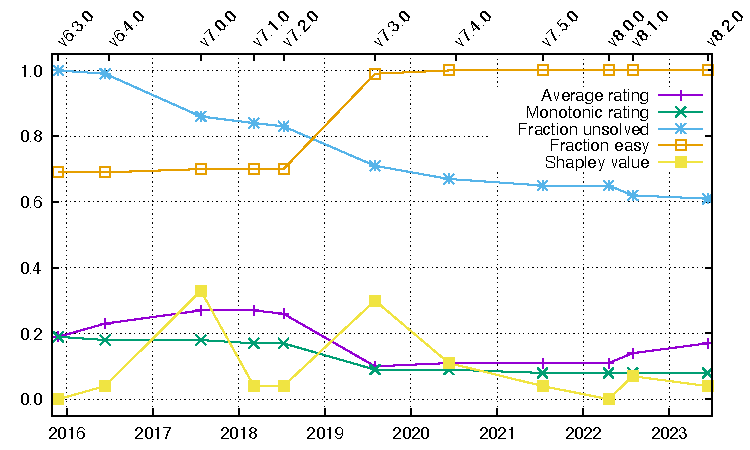
\includegraphics[width=\textwidth]{Plots/GNUPlots/CNF_EPR.pdf}
  \vspace*{-2em}
  \caption{{\tt CNF\_*\_EPR\_*}}
  \label{Plot_CNF_EPR}
\end{minipage}
\begin{minipage}[t]{.49\textwidth}
  \centering
  \includegraphics[width=\textwidth]{Plots/GNUPlots/CNF_UNS_RFO_UEQ.pdf}
  \vspace*{-2em}
  \caption{{\tt CNF\_UNS\_RFO\_PEQ\_UEQ}}
  \label{Plot_CNF_UEQ}
\end{minipage}
\begin{minipage}[t]{.49\textwidth}
  \centering
  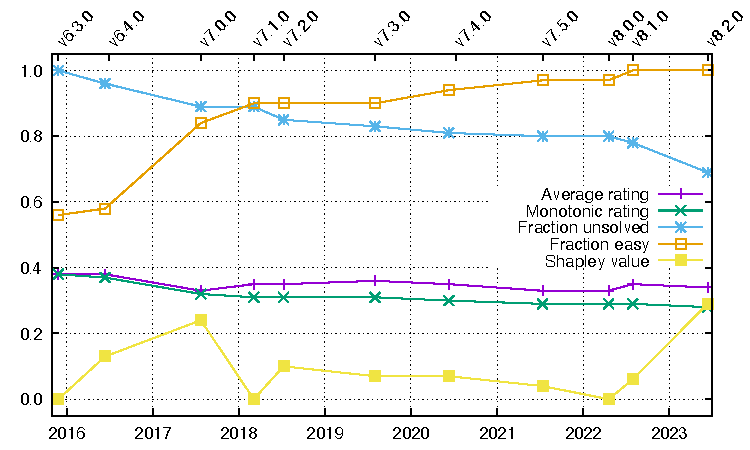
\includegraphics[width=\textwidth]{Plots/GNUPlots/CNF_UNS_RFO_NUE.pdf}
  \vspace*{-2em}
  \caption{{\tt CNF\_UNS\_RFO\_*\_NUE}}
  \label{Plot_CNF_UNS}
\end{minipage}
\begin{minipage}[t]{.49\textwidth}
  \centering
  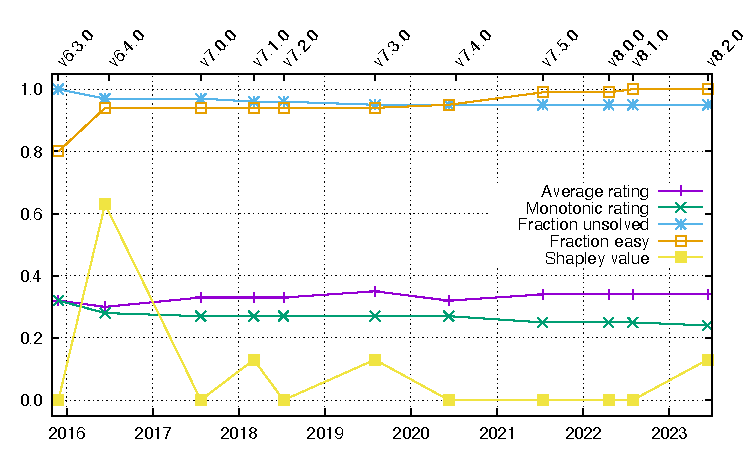
\includegraphics[width=\textwidth]{Plots/GNUPlots/CNF_SAT_RFO.pdf}
  \vspace*{-2em}
  \caption{{\tt CNF\_SAT\_RFO\_*}}
  \label{Plot_CNF_SAT}
\end{minipage}
\end{figure}

Commentary for FOF.

\begin{figure}[h!]
\centering
\begin{minipage}[t]{.49\textwidth}
  \centering
  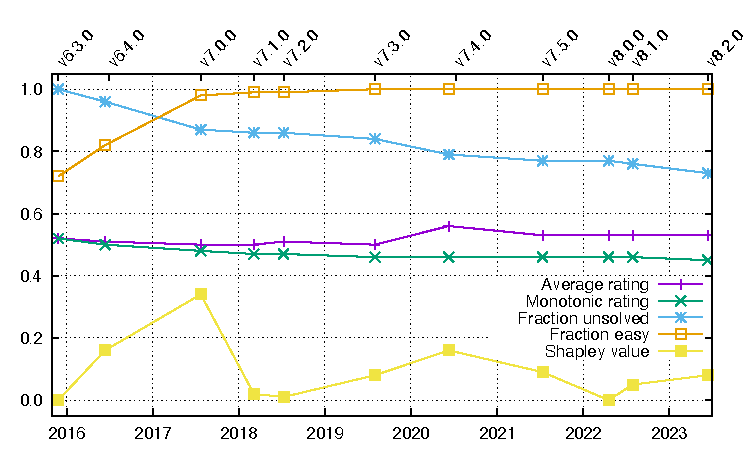
\includegraphics[width=\textwidth]{Plots/GNUPlots/FOF_THM_RFO.pdf}
  \vspace*{-2em}
  \caption{{\tt FOF\_THM\_RFO\_*}}
  \label{Plot_FOF_THM}
\end{minipage}
\begin{minipage}[t]{.49\textwidth}
  \centering
  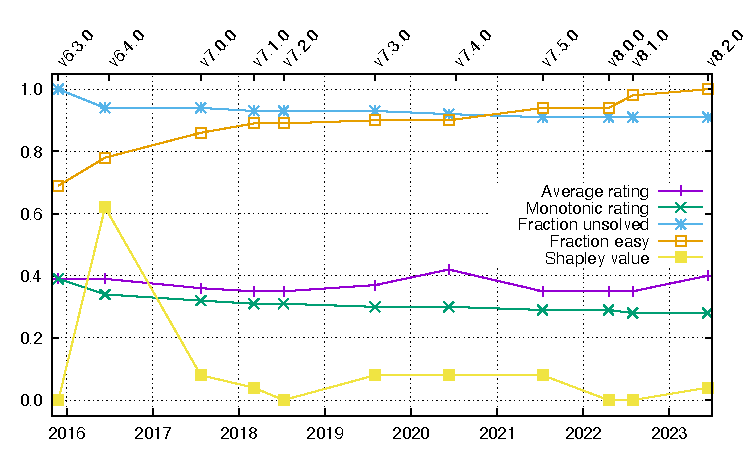
\includegraphics[width=\textwidth]{Plots/GNUPlots/FOF_CSA_SAT_RFO.pdf}
  \vspace*{-2em}
  \caption{{\tt FOF\_\{CSA,SAT\}\_RFO\_*}}
  \label{Plot_FOF_SAT}
\end{minipage}
\end{figure}

Commentary for TF0 and TH0.

\begin{figure}[h!]
\centering
\begin{minipage}[t]{.49\textwidth}
  \centering
  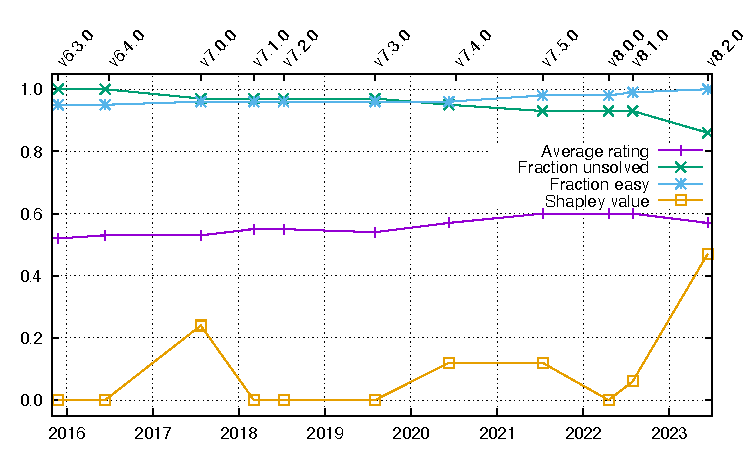
\includegraphics[width=\textwidth]{Plots/GNUPlots/TF0_THM_NAR.pdf}
  \vspace*{-2em}
  \caption{{\tt TF0\_THM\_*\_NAR}}
  \label{Plot_TF0_THM_NAR}
\end{minipage}
\begin{minipage}[t]{.49\textwidth}
  \centering
  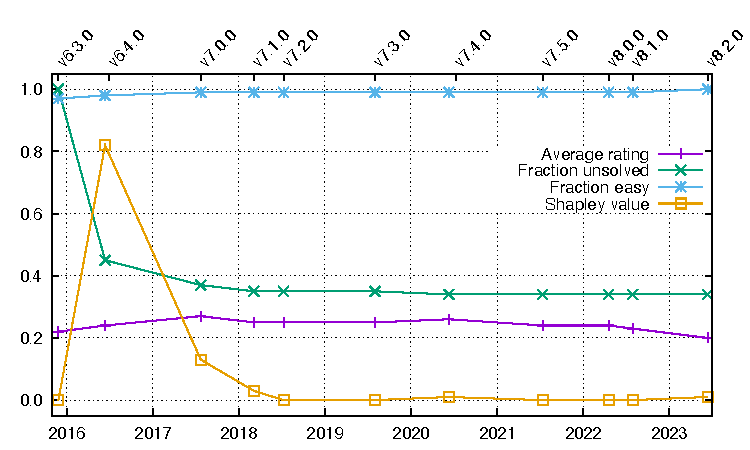
\includegraphics[width=\textwidth]{Plots/GNUPlots/TF0_THM_ARI.pdf}
  \vspace*{-2em}
  \caption{{\tt TF0\_THM\_*\_ARI}}
  \label{Plot_TF0_THM_ARI}
\end{minipage}
% \end{figure}
% \begin{figure}[ht!]
% \centering
\begin{minipage}[t]{.49\textwidth}
  \centering
  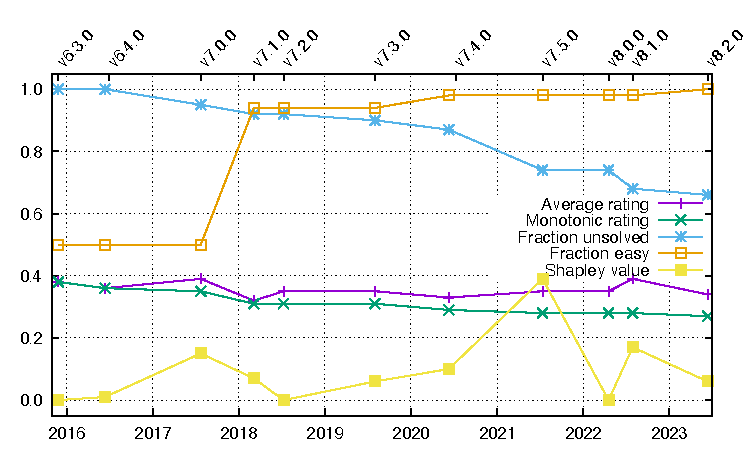
\includegraphics[width=\textwidth]{Plots/GNUPlots/TH0_THM_NAR.pdf}
  \vspace*{-2em}
  \caption{{\tt TH0\_THM\_*\_NAR}}
  \label{Plot_TH0_THM_NAR}
\end{minipage}
%\begin{minipage}[t]{.49\textwidth}
%  \centering
%  \includegraphics[width=\textwidth]{Plots/GNUPlots/ALL.pdf}
%  \vspace*{-2em}
%  \caption{All problems}
%  \label{Plot_ALL}
%\end{minipage}
\end{figure}

In prior analysis, done at TPTP release v6.4.0 \cite{Sut17}, Figure~\ref{Ratings_v5.0.0_v6.4.0} 
was presented. 
It was noted: ``Over time, decreasing difficult ratings of individual TPTP problems provide an 
indication of progress in the field \cite{SFS01}. Figure~3 plots the average ratings for the 
14527 problems that have been unchanged in the TPTP since v5.0.0, and whose ratings have not 
been stuck at 0.00 or 1.00 since v5.0.0. The ratings generally show a downward trend - there 
has been progress!''.
The same analysis has been done now at TPTP release v8.2.0, for the 16236 problems that have been 
unchanged in the TPTP since v6.3.0, and whose ratings have not been stuck at 0.00 or 1.00 since 
v6.3.0.
The two figures' plots dovetail quite well, which gives confidence that they really are comparable
(there are some minor differences caused by the data cleaning done for this work, and recent 
refinements to the rating calculations \cite{SD23-CASC,SD24-CASC}).
The older plots show a quite clear downward trend both overall and for the four types of problems,
but the latest plots do not.
The possible reasons are discussed in the conclusion (Section~\ref{Conclusion}).

\begin{figure}[h!]
\centering
\begin{minipage}[t]{.49\textwidth}
  \centering
  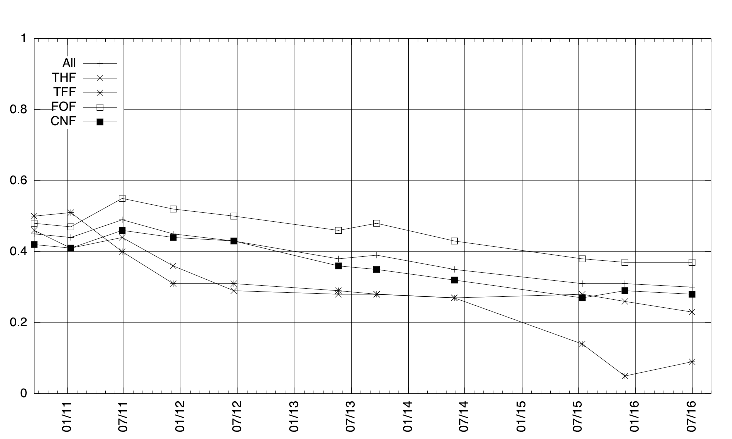
\includegraphics[width=\textwidth]{Plots/RatingsDecline_v5.0.0_v6.4.0.pdf}
  \vspace*{-2em}
  \caption{Ratings from v5.0.0 to v6.4.0}
  \label{Ratings_v5.0.0_v6.4.0}
\end{minipage}
\begin{minipage}[t]{.49\textwidth}
  \centering
  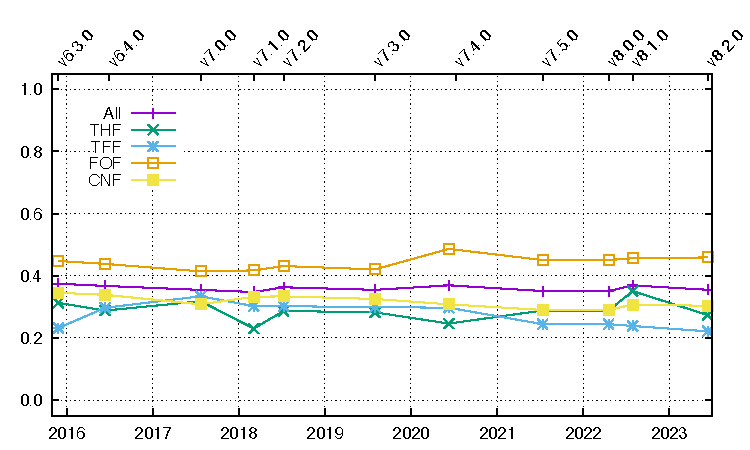
\includegraphics[width=\textwidth]{Plots/RatingsDecline_v6.3.0_v8.2.0.pdf}
  \vspace*{-2em}
  \caption{Ratings from v6.3.0 to v8.2.0}
  \label{Ratings_v6.3.0_v8.2.0}
\end{minipage}
\end{figure}

%--------------------------------------------------------------------------------------------------
\section{Conclusion}
\label{Conclusion}

This paper 

The analyses have shown progress in the last eight years, in some aspects. 
There have been some first solutions of problems that are of direct interest to humans, 
a quite large number of first ATP solutions of problems from the TPTP, and 
some noteworthy improvements in individual ATP systems.
The big picture is less bright (at least in terms of analysis of the problem difficulty ratings).
While the monotonized ratings necessarily go down, the trend is not dramatic, and the raw
ratings are generally stable.
This is in contrast to the clearly decreasing ratings from 2011 to 2016.
The reasons for this apparently slow progress are not definitely known, but we have thought of 
the following possible reasons:
\begin{itemize}
\item Systems gaining breadth of capability at the expense of depth, e.g., 
      E -- Only CNF and FOF up to 2015, added TF0 in 2017 \cite{SCV19}, TX0 and TH0 in 2019 
           \cite{VB+19};
      iProver -- Only CNF and FOF up to 2015, added TF0 with arithmetic in 2021 (unpublished);
      Vampire -- Only CNF, FOF, TF0(A) up to 2015, added THF, TXF, TF1 in ???? \cite{}.
\item New systems that take new approaches, solving different subsets of SPCs, e.g.,
      CSE\_E \cite{XL+18} -- Added in 2018, combines the S-CS calculus with E;
      Zipperposition \cite{BB+21} -- Added in 2019, extends superposition to higher-order logic;
      Twee \cite{Sma21} -- Added in 2018, solves CNF and FOF problems by transformation to UEQ.
\item Time spent on machine learning based techniques, for 
      axiom selection, e.g., \cite{Urb06,KB14}, 
      given clause selection, e.g., \cite{JU17-CICM,CA+21,AA+22-ML,MS23}), 
      learning for large problem corpora, e.g., \cite{KM+14,JU19,BL+19-ICML}, 
      and recently use of large language models to improve ATP performance \cite{WX+23,AS+23}.
\item SMT solvers have been in existence since the late 1970s \cite{NO79}, and blossomed fully
      in the early 2000s.
      Since then there has been ever-increasing emphasis on SMT solving, with ATP systems being 
      adapted to solving SMT problems, e.g., Vampire has been into SMT-COMP since 2016, and
      iProver since 2021.
      This is all good work, but has possibly diverted developer energy from ATP to SMT.
\item In \cite{SD24-CASC} it was noted that CASC might be causing incremental development of ATP
      systems.
      This concern has been expressed as far back as CASC-JC in 2001 \cite{PSS02}.
      In response to this concern CASC-J12 will have a new ICU (I Challenge yoU) division that
      focusses on solving hard problems rather than solving more problems, hoping to stimulate
      new developments and progress.
\end{itemize}

Ongoing and future work includes~\ldots

%--------------------------------------------------------------------------------------------------
\bibliographystyle{splncs04}
\bibliography{Bibliography}
%--------------------------------------------------------------------------------------------------
\end{document}
